\section{Hypotheses}

$\mathcal{H}_1$: RJCB expects that the inference error is lowest when the true
tree is generated under MBD parameter settings without multiple-births, i.e
$nu = 0 \vee q = 0$. For such parameters settings, the
true is in practice generated by a BD model, which
matches the tree prior used in inference. Without a mismatch between
true tree prior and assumed tree prior, this source of errors will be absent,
where the other two sources of errors (stochasticity in the
simulation of the alignment and the MCMC algorithm) 
will remain the same. \richel{figure 1a and b}

$\mathcal{H}_2$: RJCB expects that, on average, the inference error is highest for
parameter settings with a higher percentage of multiple-births,
i.e. $nu > 0 \wedge q > 0$, as for these settings, 
the mismatch between the the speciation model that
generated the true tree (which is profoundly-MB MBD) is biggest with
the tree prior assumed to be generative (which is BD). \richel{figure 1a and b}

$\mathcal{H}_3$: RJCB expects that the inference error is higher for true trees
with a higher percentage of species observably generated in an MB event,
regardless of the MBD parameters.
These multiple-born species are one of the three (and the most 
interesting) sources of error, as a BD model -as a feature- will never
infer a co-occuring speciation event. \richel{figure 2}

$\mathcal{H}_4$: RJCB expects that, on average, the inference error is equal for
parameter settings with an equal $\lambda$, $\nu$ and $q$, i.e. extinction
has no effect on the error made, because extinction affects all species equally. 
\richel{figure 1a and b, or a new figure}
\giovanni{A higher extinction rate increases variance and tends to reduce to number of taxa in the tree. According to your other hypotheses (e.g. H5) these effects do affect the inference. Therefore you need to adjust for these variables to prove your hypothesis.}

$\mathcal{H}_5$: RJCB expects that an increased number of taxa
has a negative effect on the variance of the errors made, as there
is more information available to base inference on.
\richel{figure 3}

$\mathcal{H}_6$: RJCB expects that an increased extinction rate
increases the variance of the errors made,
due to the decrease of the number of taxa, reducing the amount of information
to base inference on.
\richel{figure 4}

$\mathcal{H}_7$: RJCB expects that the nLTT statistic between a true and twin
tree at the start of the pipeline,
will correlate strongly with the difference
between the highest posterior density (HPD) of the 
errors of the true and twin tree 
generated at the end of the pipeline. 
This hypothesis
stems from the idea of assuming a setup without noise; that is, with
a DNA alignment of infinite length. From such a DNA alignment 
with infinite information, the MCMC
is able to infer the close-to-correct phylogeny.
\richel{if this is true, we can use this shortcut (instead of running
multiple pirouette replicates) to draw stronger conclusions}
\giovanni{I can agree with the principle. However there are also other factors that you might overlook with such approximation. It might be useful, though, for a fast comparison to have a preliminary idea, if the hypothesys will be confirmed by the experiment.}
\richel{figure 5}

\begin{figure}[!htbp]
  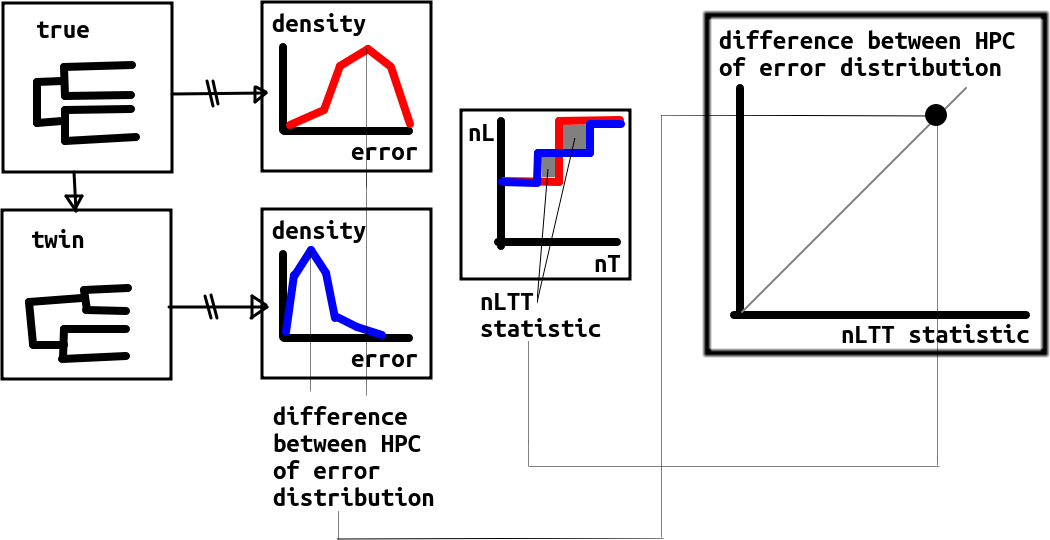
\includegraphics[width=\textwidth]{20191126_nltt_as_proxy.png}
  \caption{
    The nLTT statistic between true and twin tree correlates strongly
    with the difference between (the highest posterior density
    of) the errors of the true and twin tree.
  }
  \label{fig:nltt_as_proxy}
\end{figure}

$\mathcal{H}_8$: RJCB expects that for settings without extinctions,
the candidate model with JC69, strict and Yule will come up as the best
model most, as that model is the generative model, where the HKY, strict, BD
will be seleted least, as both its site and tree model are needlessly complex.
For settings with extinctions, RJCB predict HKY, strict and Yule will come up 
as the worst model mostly, as it uses both an incorrect site model and incorrect
tree model. \richel{I would enjoy a hypothesis of actual biological relevance for the
candidate models. If we cannot devise one, I suggest to remove the
use of candidate models}

$\mathcal{H}_9$: GL expects a positive correlation between $\nu \, q(1-q)$ and the error made by the inference process. This is due to the fact that this factor expresses the variance of the underlying binomial distribution that regulates multiple births events.